\documentclass{article}

\usepackage{graphicx} %[pdftex] OR [dvips]
\usepackage{fullpage}
\usepackage{float}
\usepackage{titling}
\setlength{\droptitle}{-6em}

\newcommand{\ghcfile}[1]{\textsl{#1}}

\title{Implementing Backpack}

\begin{document}

\maketitle

The purpose of this document is to describe an implementation path
for Backpack~\cite{Kilpatrick:2014:BRH:2535838.2535884} in GHC\@.

We start off by outlining the current architecture of GHC, ghc-pkg and Cabal,
which constitute the existing packaging system.  We then state what our subgoals
are, since there are many similar sounding but different problems to solve.  Next,
we describe the ``probably correct'' implementation plan, and finish off with
some open design questions.  This is intended to be an evolving design document,
so please contribute!

\section{Current packaging architecture}

The overall architecture is described in Figure~\ref{fig:arch}.

\begin{figure}[H]
    \center{\scalebox{0.8}{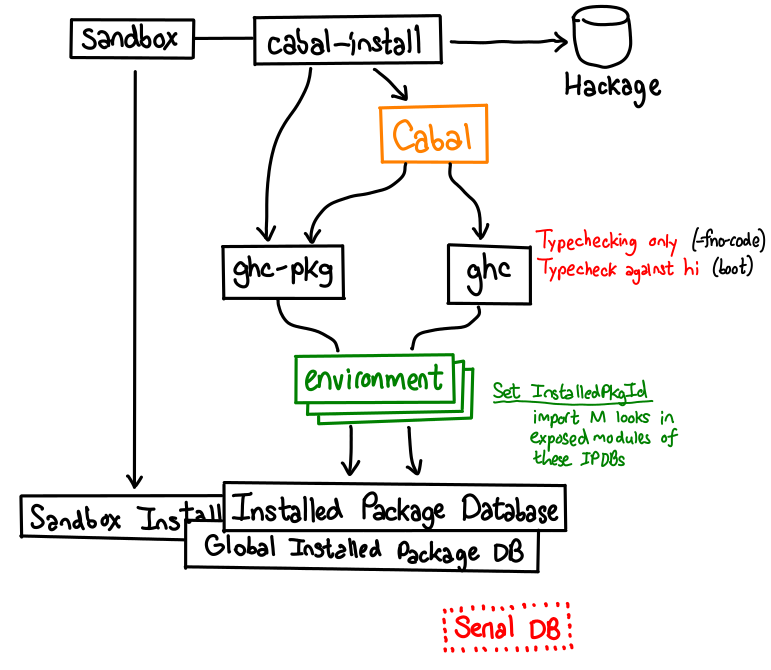
\includegraphics{arch.png}}}
\label{fig:arch}\caption{Architecture of GHC, ghc-pkg and Cabal. Green bits indicate additions from upcoming IHG work, red bits indicate additions from Backpack.  Orange indicates a Haskell library.}
\end{figure}

Here, arrows indicate dependencies from one component to another.  Color
coding is as follows: orange components are libaries, green components
are to be added with the IHG work, red components are to be added with
Backpack.  (Thus, black and orange can be considered the current)

\subsection{Installed package database}

Starting from the bottom, we have the \emph{installed package database}
(actually a collection of such databases), which stores information
about what packages have been installed are thus available to be
compiled against.  There is both a global database (for the system
administrator) and a local database (for end users), which can be
updated independently.  One way to think about the package database
is as a \emph{cache of object code}.  In principle, one could compile
any piece of code by repeatedly recompiling all of its dependencies;
the installed package database describes when this can be bypassed.

\begin{figure}[H]
    \center{\scalebox{0.8}{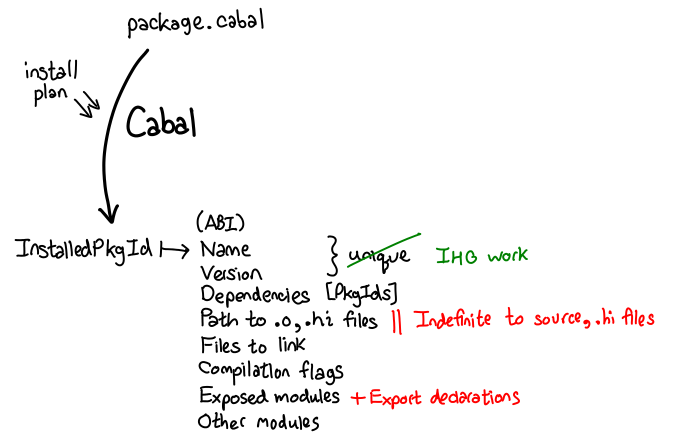
\includegraphics{pkgdb.png}}}
\label{fig:pkgdb}\caption{Anatomy of a package database.}
\end{figure}

In Figure~\ref{fig:pkgdb}, we show the structure of a package database.
The installed package are created from a Cabal file through the process
of dependency resolution and compilation.  In database terms, the primary key
of a package database is the InstalledPackageId
(Figure~\ref{fig:current-pkgid}).  This ID uniquely identifies an
instance of an installed package.  The PackageId omits the ABI hash and
is used to qualify linker exported symbols: the current value of this
parameter is communicated to GHC using the \verb|-package-id| flag.

In principle, packages with different PackageIds should be linkable
together in the same compiled program, whereas packages with the same
PackageId are not (even if they have different InstalledPackageIds).  In
practice, GHC is currently only able to select one version of a package,
as it clears out all old versions of the package in
\ghcfile{compiler/main/Package.lhs}:applyPackageFlag.

\begin{figure}
    \center{\begin{tabular}{r l}
        PackageId & package name, package version \\
        InstalledPackageId & PackageId, ABI hash \\
    \end{tabular}}
\label{fig:current-pkgid}\caption{Current structure of package identifiers.}
\end{figure}

The database entry itself contains the information from the installed package ID,
as well as information such as what dependencies it was linked against, where
its compiled code and interface files live, its compilation flags, what modules
it exposes, etc.  Much of this information is only relevant to Cabal; GHC
uses a subset of the information in the package database.

\subsection{GHC}

The two programs which access the package database directly are GHC
proper (for compilation) and ghc-pkg (which is a general purpose
command line tool for manipulating the database.)  GHC relies on
the package database in the following ways:

\begin{itemize}
    \item It imports the local and global package databases into
        its runtime database, and applies modifications to the exposed
        and trusted status of the entries via the flags \verb|-package|
        and others (\ghcfile{compiler/main/Packages.lhs}).  The internal
        package state can be seen at \verb|-v4| or higher.
    \item It uses this package database to find the location of module
        interfaces when it attempts to load the module info of an external
        module (\ghcfile{compiler/iface/LoadIface.hs}).
\end{itemize}

GHC itself performs a type checking phase, which generates an interface
file representing the module (so that later invocations of GHC can load the type
of a module), and then after compilation projects object files and linked archives
for programs to use.

\paragraph{Original names} Original names are an important design pattern
in GHC\@.
Sometimes, a name can be exposed in an hi file even if its module
wasn't exposed. Here is an example (compiled in package R):

\begin{verbatim}
module X where
    import Internal (f)
    g = f

module Internal where
    import Internal.Total (f)
\end{verbatim}

Then in X.hi:

\begin{verbatim}
g = <R.id, Internal.Total, f> (this is the original name)
\end{verbatim}

(The reason we refer to the package as R.id is because it's the
full package ID, and not just R).

\subsection{hs-boot}

\verb|hs-boot| is a special mechanism used to support recursive linking
of modules within a package, today.  Suppose I have a recursive module
dependency between modules and A and B. I break one of\ldots

(ToDo: describe how hs-boot mechanism works)

\subsection{Cabal}

Cabal is the build system for GHC, we can think of it as parsing a Cabal
file describing a package, and then making (possibly multiple)
invocations to GHC to perform the appropriate compilation.  What
information does Cabal pass onto GHC\@?  One can get an idea for this by
looking at a prototypical command line that Cabal invokes GHC with:

\begin{verbatim}
ghc --make
    -package-name myapp-0.1
    -hide-all-packages
    -package-id containers-0.9-ABCD
    Module1 Module2
\end{verbatim}

There are a few things going on here.  First, Cabal has to tell GHC
what the name of the package it's compiling (otherwise, GHC can't appropriately
generate symbols that other code referring to this package might generate).
There are also a number of commands which configure its in-memory view of
the package database (GHC's view of the package database may not directly
correspond to what is on disk).  There's also an optimization here: in principle,
GHC can compile each module one-by-one, but instead we use the \verb|--make| flag
because this allows GHC to reuse some data structures, resulting in a nontrivial
speedup.

(ToDo: describe cabal-install/sandbox)

\section{Goals}

There are actually a number of different goals we have for modifying the
packaging system, some of which are subsets of the Backpack system.

\begin{itemize}
    \item As a prerequisite, support multiple instances of containers-2.9 \emph{in the
        package database}.  These instances may be compiled against
        different dependencies, have the same dependencies but different
        source files (as when a package is being developed), or be
        compiled with different options.  It is less important to allow
        these instances to be linkable together.\footnote{Actually, I think
        this is completely orthogonal to Backpack, since we are going to treat
        dependencies as part of the package ID, so they would be considered
        separate entries in the package database anyway.}

    \item Support typechecking a library against a module interface
        as opposed to an actual implementation.  This would be useful
        for moving towards a model where Cabal package dependency versions
        are replaced with proper signature packages. %  See Section~\ref{sec:signature-packages} for more details.

    \item Support compiling the aforementioned libraries with actual implementations.
        It is \emph{not} a goal to be able to compile a library while only
        partially providing dependencies, and it is low priority to support
        mutually recursive implementations of these implementations.

        \iffalse%
    \item Support insertion of backwards compatibility shims for packages
        that are using old versions of packages, so that you can continue
        using them without having to patch them manually.  This is a
        stylized use-case of Backpack features.  See Section~LINKME for
        more details.

    \item Some easy-to-implement subset of the functionality provided by
        packages with holes (Backpack proper).  This includes support
        of linking an executable containing multiple packages with the
        same package name but different PackageIds.
        \fi
\end{itemize}

A lower priority goal is to actually allow multiple instances of
containers-2.9 to be linked together in the same executable
program.\footnote{In particular, this requires changes to how linker
symbols are assigned. However, this feature is important to
implement a number of Backpack features.}

A \emph{non-goal} is to allow users to upgrade upstream libraries
without recompiling downstream. This is an ABI concern and we're not
going to worry about it.

\section{Aside: Recent IHG work}\label{sec:ihg}

The IHG project has allocated some funds to relax the package instance
constraint in the package database, so that multiple instances can be
stored, but now the user of GHC must explicitly list package-IDs to be
linked against.  In the far future, it would be expected that tools like
Cabal automatically handle instance selection among a large number of
instances, but this is subtle and so this work is only to do some
foundational work, allowing a package database to optionally relax the
unique package-version requirement, and utilize environment files to
select which packages should be used.  See Duncan's email for more
details on the proposal.

To implement this:

\begin{enumerate}

    \item Remove the ``removal step'' when registering a package (with a flag)

    \item Check \ghcfile{compiler/main/Packages.lhs}:mkPackagesState to look out for shadowing
      within a database. We believe it already does the right thing, since
      we already need to handle shadowing between the local and global database.

\end{enumerate}

Once these changes are implemented, we can program multiple instances by
using \verb|-hide-all-packages -package-id ...|, even if there is no
high-level tool support.

Actually, this concern is orthogonal to the purposes of Backpack, if
we redefine PackageId appropriately.

\paragraph{The ABI hash} Currently, InstalledPackageId
is constructed of a package, version and ABI hash
(generateRegistrationInfo in
\ghcfile{libraries/Cabal/Cabal/Distribution/Simple/Register.hs}).  The
use of an ABI hash is a bit of GHC-specific hack introduced in 2009,
intended to make sure these installed package IDs are unique.  While
this is quite clever, using the ABI is actually a bit inflexible, as one
might reasonably want to have multiple copies of a package with the same
ABI but different source code changes.\footnote{In practice, our ABIs
are so unstable that it doesn't really matter.}

In Figure~\ref{fig:proposed-pkgid}, there is an alternate logical
representation of InstalledPackageId which attempts to extricate the
notion of ABI compatibility from what actually might uniquely identify a
package beyond its PackageId.  We imagine these components to be:

\begin{itemize}
    \item A hash of the source code (so one can register different
        in-development versions without having to bump the version
        number);
    \item Compilation way (profiling? dynamic?)
    \item Compilation flags (such as compilation way, optimization,
        profiling settings)\footnote{This is a little undefined on a package bases, because in principle the flags could be varied on a per-file basis. More likely this will be approximated against the relevant fields in the Cabal file as well as arguments passed to Cabal.};
\end{itemize}

A historical note: in the 2012 GSoC project to allow multiple instances
of a package to be installed at the same time, use of \emph{random
numbers} was used to workaround the inability to get an ABI early
enough.  We are not using this plan.

\section{Infrastructural improvements}

There are some infrastructural improvements that must be made before
Backpack proper can be implemented.  These additions are described in
red in the architectural diagrams.  The current structure of this
section is to describe the additions bottom up.

\subsection{Concrete physical identity = PackageId$^*$ + Module name}\label{sec:ipi}

\begin{figure}
    \center{\begin{tabular}{r l}
        PackageId & hash of ``package name, package version, PackageIds of dependent packages'' \\
        InstalledPackageId & hash of ``PackageId, source code, way, compiler flags'' \\
    \end{tabular}}
\label{fig:proposed-pkgid}\caption{Proposed new structure of package identifiers.}
\end{figure}

In Backpack, there needs to be some mechanism for assigning
\emph{physical module identities} to modules, which are essential for
typechecking Backpack packages, since they let us tell if two types are
equal or not. In the paper, the physical identity was represented as the
package that constructed it as well as some representation of the module
source.  We can simplify this slightly: in current Cabal packages, we
require that modules always be given a package-unique logical name;
thus, physical identities can be simply represented as a PackageId plus
module name. (See \ghcfile{compiler/basicTypes/Module.lhs:Module})
In fact, this coincides with how GHC already internally handles
the problem of type equality: it appeals to an \emph{original name}
which is, presently, a PackageId and the module name.

However, with the current representation of PackageIds, this is
insufficient: a package is not just its name, but also the regular
tree representing all of its package dependencies.  Thus, we have
to adjust the representation of a PackageId so that it includes this
regular tree, as seen Figure~\ref{fig:proposed-pkgid}.  Since this
tree in general may be quite long, it needs to be shortened in some way,
such as by hashing.

And now, the complications\ldots

\paragraph{Relaxing package selection restrictions}  As mentioned
previously, GHC is unable to select multiple packages with the same
package name (but different PackageIds).  This restriction needs to be
lifted.  For backwards compatibility reasons, it's probably better to
not overload \verb|-package-id| but add a new flag, maybe \verb|-force-package-id|;
we also need to disable the old version masking behavior.  This is orthogonal
to the IHG work, which wants to allow multiple InstalledPackageIds in the
\emph{database} (here, we want to allow multiple PackageIds in compiled code).

\paragraph{Linker symbols} As we increase the amount of information in
PackageId, it's important to be careful about the length of these IDs,
as they are used for exported linker symbols (e.g.
\verb|base_TextziReadziLex_zdwvalDig_info|).  Very long symbol names
hurt compile and link time, object file sizes, GHCi startup time,
dynamic linking, and make gdb hard to use.  As such, the current plan is
to do away with full package names and versions, and instead use just a
base-62 encoded hash, perhaps with the first four characters of the package
name for user-friendliness.

Edward: I'm still partial to a short hash of the dependency bits (or
even Simon's registry of short strings to dependency trees), and keeping
everything else the same.

\paragraph{Wired-in names} One annoying thing to remember is that GHC
has wired-in names, which refer to packages without any version.  Now
these wired names also have to accomodate dependency trees. A
suggested approach is to have a fixed table from these wired names to
package IDs; alternately we can use something like the special \verb|inplace|
version number.

\paragraph{Free variables (or, what is a non-concrete physical
identity?)} Physical identities in their full generality are permitted
to have free variables, which represent holes.  Handling this is a
tricky question, and we defer it to Section~\ref{sec:typechecking-indefinite}, when
we talk about packages with holes.

\subsection{Exposed modules should allow external modules}\label{sec:reexport}

In Backpack, the definition of a package consists of a logical context,
which maps logical module names to physical module names.  These do not
necessarily coincide, since some physical modules may have been defined
in other packages and mixed into this package.  This mapping specifies
what modules other packages including this package can access.
However, in the current installed package database, we have exposed-modules which
specify what modules are accessible, but we assume that the current
package is responsible for providing these modules.

To implement Backpack, we have to extend this exposed-modules (``Export declarations''
on Figure~\ref{fig:pkgdb}).  Rather
than a list of logical module names, we provide a new list of tuples:
the exported logical module name and original physical module name (this
is in two parts: the InstalledPackageId and the original module name).
For example, an traditional module export is simply (Name, my-pkg-id, Name);
a renamed module is (NewName, my-pkg-id, OldName), and an external module
is (Name, external-pkg-id, Name).

As an example:

\begin{verbatim}
package P where
    M = ...
    N = ...
package Q (M, R, T)
    include P (N -> R)
    T = ...
\end{verbatim}

And now if we look at Q\@:

\begin{verbatim}
exposed-modules:
        <M, P.id, M>
        <R, P.id, N>
        <T, Q.id, T>
\end{verbatim}

When we compile Q, and the interface file gets generated, we have
to generate identifiers for each of the exposed modules.  These should
be calculated to directly refer to the ``original name'' of each them;
so for example M and R point directly to package P, but they also
include the original name they had in the original definition.

\section{Simplifying Backpack}\label{sec:simplifying-backpack}

Backpack as currently defined always requires a \emph{shaping} pass,
which calculates the shapes of all modules defined in a package.
The shaping pass is critical to the solution of the double-vision problem
in recursive module linking, but it also presents a number of unpalatable
implementation problems:

\begin{itemize}

    \item \emph{Shaping is a lot of work.} A module shape specifies the
        providence of all data types and identifiers defined by a
        module. To calculate this, we must preprocess and parse all
        modules, even before we do the type-checking pass.

    \item \emph{Shaping must be done upfront.} In the current Backpack
        design, all shapes must be computed before any typechecking can
        occur.  While performing the shaping pass upfront is necessary
        in order to solve the double vision problem (where a module
        identity may be influenced by later definitions), it also means
        that either GHC must compile an entire package in one go, or it
        must first do a shaping pass, and then revisit every module and
        compile them proper.  Nor is it (easily) possible to skip the
        shaping pass when it is unnecessary, as one might expect to be
        the case in the absence of mutual recursion.  Shaping is not
        a ``pay as you go'' language feature.

    \item \emph{GHC can't compile all programs shaping accepts.}  Shaping
        accepts programs that GHC, with its current hs-boot mechanism, cannot
        compile.  In particular, GHC requires that any data type or function
        in a signature actually be \emph{defined} in the module corresponding
        to that file (i.e., an original name can be assigned to these entities
        immediately.)  Shaping permits unrestricted exports to implement
        modules; this shows up in the formalism as $\beta$ module variables.

    \item \emph{Shaping encourages inefficient program organization.}
        Shaping is designed to enable mutually recursive modules, but as
        currently implemented, mutual recursion is less efficient than
        code without recursive dependencies. Programmers should avoid
        this code organization, except when it is absolutely necessary.

    \item \emph{GHC is architecturally ill-suited for shaping.}  Shaping
        implies that GHC's internal concept of an ``original name'' be
        extended to accommodate module variables.  This is an extremely
        invasive change to all aspects of GHC, since the original names
        assumption is baked quite deeply into the compiler.

\end{itemize}

To be clear, the shaping pass is fundamentally necessary for some
Backpack packages.  Here is the example which convinced Simon:

\begin{verbatim}
package p where
    A :: [data T; f :: T -> T]
    B = [export T(MkT), h; import A(f); data T = MkT; h x = f MkT]
    A = [export T(MkT), f, h; import B; f MkT = MkT]
\end{verbatim}

The key to this example is that B \emph{may or may not typecheck} depending
on the definition of A. Because A reexports B's definition T, B will
typecheck; but if A defined T on its own, B would not typecheck.  Thus,
we \emph{cannot} typecheck B until we have done some analysis of A (the
shaping analysis!)

So, if we want to jettison the shaping analysis, we'd like a subset
of Backpack which does not allow mutually recursive modules.
Here is a programming discipline which does just that, which we will call the \textbf{linking restriction}: \emph{Module implementations must be declared before
signatures.}  Formally, this restriction modifies the rule for merging
polarized module shapes ($\widetilde{\tau}_1^{m_1} \oplus \widetilde{\tau}_2^{m_2}$) so that
$\widetilde{\tau}_1^- \oplus \widetilde{\tau}_2^+$ is always undefined.\footnote{This seemed to be the crispest way of defining the restriction, although this means an error happens a bit later than I'd like it to: I'd prefer if we errored while merging logical contexts, but we don't know what is a hole at that point.}

Here is an example of the linking restriction. Consider these two packages:

\begin{verbatim}
package random where
    System.Random = [ ... ].hs

package monte-carlo where
    System.Random :: ...
    System.MonteCarlo = [ ... ].hs
\end{verbatim}

Here, random is a definite package which may have been compiled ahead
of time; monte-carlo is an indefinite package with a dependency
on any package which provides \verb|System.Random|.

Now, to link these two applications together, only one ordering
is permissible:

\begin{verbatim}
package myapp where
    include random
    include monte-carlo
\end{verbatim}

If myapp wants to provide its own random implementation, it can do so:

\begin{verbatim}
package myapp2 where
    System.Random = [ ... ].hs
    include monte-carlo
\end{verbatim}

In both cases, all of \verb|monte-carlo|'s holes have been filled in by the time
it is included.  The alternate ordering is not allowed.

Why does this discipline prevent mutually recursive modules?  Intuitively,
a hole is the mechanism by which we can refer to an implementation
before it is defined; otherwise, we can only refer to definitions which
preceed our definition. If there are never any holes \emph{which get filled},
implementation links can only go backwards, ruling out circularity.

It's easy to see how mutual recursion can occur if we break this discipline:

\begin{verbatim}
package myapp2 where
    include monte-carlo
    System.Random = [ import System.MonteCarlo ].hs
\end{verbatim}

\subsection{Typechecking of definite modules without shaping}

If we are not carrying out a shaping pass, we need to be able to calculate
$\widetilde{\Xi}_{\mathsf{pkg}}$ on the fly.  In the case that we are
compiling a package---there will be no holes in the final package---we
can show that shaping is unnecessary quite easily, since with the
linking restriction, everything is definite from the get-go.

Observe the following invariant: at any given step of the module
bindings, the physical context $\widetilde{\Phi}$ contains no
holes.  We can thus conclude that there are no module variables in any
type shapes.  As the only time a previously calculated package shape can
change is due to unification, the incrementally computed shape is in
fact the true one.

As far as the implementation is concerned, we never have to worry
about handling module variables; we only need to do extra typechecks
against (renamed) interface files.

\subsection{Compilation of definite modules}\label{sec:compiling-definite}

Of course, we still have to compile the code,
and this includes any subpackages which we have mixed in the dependencies
to make them fully definite.  Let's take the following package as an example:

\begin{verbatim}
package pkg-a where
    A = ...
package pgk-b where -- indefinite package
    A :: ...
    B = [ b = ... ]
package pkg-c where
    include pkg-a
    include pkg-b
\end{verbatim}

There seem to be two schools of thought for how compilation should proceed.

\paragraph{The ``downstream'' proposal}  This is Simon's favorite
proposal.  Because of the linking invariant, if we traverse the Backpack
specification, any given module we need to compile will have all of its
dependencies compiled (since it could only depend on the dependency if
there was a signature, and the signature could not have been linked
unless it was implemented previously.)  So we just go ahead and compile
everything one-by-one while traversing the package tree, as if the
package was a single big package.  (Of course, if we encounter a
definite package, don't bother recompiling it; just use it directly.)
In particular, we maintain the invariant that any code generated will
export symbols under the current package's namespace.  So the identifier
\verb|b| in the example becomes a symbol \verb|pkg-c_pkg-b_B_b| rather
than \verb|pkg-b_B_b| (package subqualification is necessary because
package C may define its own B module after thinning out the import.)

One big problem with this proposal is that it doesn't implement applicative
semantics.  If there is another package:

\begin{verbatim}
package pkg-d where
    include pkg-a
    include pkg-b
\end{verbatim}

this will generate its own instance of B, even though it should be the same
as C.  Simon was willing to entertain the idea that, well, as long as the
type-checker is able to figure out they are the same, then it might be OK
if we accidentally generate two copies of the code (provided they actually
are the same).

\paragraph{The ``upstream'' proposal}
The problem with the ``downstream'' proposal is that it always recompiles
all of the indefinite parts of the package, even if some of them should
be shared in some sense.  Hypothetically, a fully linked version of an
indefinite package should be considered a package in its own right
(in particular, it is associated with a physical module identity in Backpack).
So all we need to do is store these installed packages somewhere, probably
the local package database.  If we recompile the same dependency chain,
the installed package can be simply reused.  These products do not have
to be exposed.

One problem with this proposal is in this example:

\begin{verbatim}
package myapp2 where
    System.Random = [ ... ].hs
    include monte-carlo
\end{verbatim}

Here, monte-carlo depends on a ``subpart of the myapp2 package'', and it's
not entirely clear how monte-carlo should be represented in the installed
package database: should myapp2 be carved up into pieces so that subparts
of its package description can be installed to the database?

Another reason you might not be so keen about this proposal is the fact
that we have to hit the package database, despite the fact that these
are all ostensibly local build products. (But perhaps not!)

\subsection{Typechecking of indefinite modules}\label{sec:typechecking-indefinite}

When we are typechecking a package that contains some holes, some extra
care must be taken.  We can no longer assume that there are no holes in
the physical context, and while these holes will never be linked against
a physical implementation, they may be linked against other signatures.
(Note: while disallowing signature linking would solve our problem, it
would disallow a wide array of useful instances of signature reuse, for
example, a package mylib that implements both mylib-1x-sig and mylib-2x-sig.)

With holes, we must handle module variables, and we sometimes must unify them:

\begin{verbatim}
package p where
    A :: [ data A ]
package q where
    A :: [ data A ]
package r where
    include p
    include q
\end{verbatim}

In this package, it is not possible to a priori assign original names to
module A in p and q, because in package r, they should have the same
original name.  When signature linking occurs, unification may occur,
which means we have to rename all relevant original names. (A similar
situation occurs when a module is typechecked against a signature.)

An invariant which would be nice to have is this: when typechecking a
signature or including a package, we may apply renaming to the entities
being brought into context.  But once we've picked an original name for
our entities, no further renaming should be necessary. (Formally, in the
unification for semantic object shapes, apply the unifier to the second
shape, but not the first one.)

However, there are plenty of counterexamples here:

\begin{verbatim}
package p where
    A :: [ data A ]
    B :: [ data A ]
    M = ...
    A = B
\end{verbatim}

In this package, does module M know that A.A and B.A are type equal?  In
fact, the shaping pass will have assigned equal module identities to A
and B, so M \emph{equates these types}, despite the aliasing occurring
after the fact.

We can make this example more sophisticated, by having a later
subpackage which causes the aliasing; now, the decision is not even a
local one (on the other hand, the equality should be evident by inspection
of the package interface associated with q):

\begin{verbatim}
package p where
    A :: [ data A ]
    B :: [ data A ]
package q where
    A :: [ data A ]
    B = A
package r where
    include p
    include q
\end{verbatim}

Another possibility is that it might be acceptable to do a small shaping
pass, without parsing modules or signatures, \emph{simply} looking at
names and aliases.  But logical names are not the only mechanism by
which unification may occur:

\begin{verbatim}
package p where
    C :: [ data A ]
    A = [ data A = A ]
    B :: [ import A(A) ]
    C = B
\end{verbatim}

It is easy to conclude that the original names of C and B are the same.  But
more importantly, C.A must be given the original name of p:A.A.  This can only
be discovered by looking at the signature definition for B. In any case, it
is worth noting that this situation parallels the situation with hs-boot
files (although there is no mutual recursion here). See Section~\ref{sec:hs-boot-restirct}
for more details.

\paragraph{Hey, these signature imports are kind of tricky\ldots}

When signatures and modules are interleaved, the interaction can be
complex.  Here is an example:

\begin{verbatim}
package p where
    C :: [ data A ]
    M = [ import C; ... ]
    A = [ import M; data A = A ]
    C :: [ import A(A) ]
\end{verbatim}

Here, the second signature for C refers to a module implementation A
(this is permissible: it simply means that the original name for p:C.A
is p:A.A).  But wait! A relies on M, and M relies on C. Circularity?
Fortunately not: a client of package p will find it impossible to have
the hole C implemented in advance, since they will need to get their hands on module
A\ldots but it will not be defined prior to package p.

In any case, however, it would be good to emit a warning if a package
cannot be compiled without mutual recursion.

\subsection{Installing indefinite packages}\label{sec:installing-indefinite}

If an indefinite package contains no code at all, we only need
to install the interface file for the signatures.  However, if
they include code, we must provide all of the
ingredients necessary to compile them when the holes are linked against
actual implementations.  (Figure~\ref{fig:pkgdb})

\paragraph{Source tarball or preprocessed source?}  What is the representation of the source that is saved is.  There
are a number of possible choices:

\begin{itemize}
    \item The original tarballs downloaded from Hackage,
    \item Preprocessed source files,
    \item Some sort of internal, type-checked representation of Haskell code (maybe the output of the desugarer).
\end{itemize}

Storing the tarballs is the simplest and most straightforward mechanism,
but we will have to be very certain that we can recompile the module
later in precisely the same we compiled it originally, to ensure the hi
files match up (fortunately, it should be simple to perform an optional
sanity check before proceeding.) The appeal of saving preprocessed
source, or even the IRs, is that this is conceptually this is exactly
what an indefinite package is: we have paused the compilation process
partway, intending to finish it later.  However, our compilation strategy
for definite packages requires us to run this step using a \emph{different}
choice of original names, so it's unclear how much work could actually be reused.

\subsection{Restricted recursive modules ala hs-boot}\label{sec:hs-boot-restrict}

It should be possible to support GHC-style mutual recursion using the
Backpack formalism immediately using hs-boot files.  However, to avoid
the need for a shaping pass, we must adopt an existing constraint that
already applies to hs-boot files: \emph{at the time we define a signature,
we must know what the original name for all data types is}.  We then
compile modules as usual, but compiling against the signature as if it
were an hs-boot file.

(ToDo: Figure out why this eliminates the shaping pass)

Compiling packages in this way gives the tantalizing possibility
of true separate compilation: the only thing we don't know is what the actual
package name of an indefinite package will be, and what the correct references
to have are.  This is a very minor change to the assembly, so one could conceive
of dynamically rewriting these references at the linking stage.

\section{Implementation plan}

\section{Open questions}\label{sec:open-questions}

Here are open problems about the implementation which still require
hashing out.

\begin{itemize}

    \item In Section~\ref{sec:simplifying-backpack}, we argued that we
        could implement Backpack without needing a shaping pass. We're
        pretty certain that this will work for typechecking and
        compiling fully definite packages with no recursive linking, but
        in Section~\ref{sec:typechecking-indefinite}, we described some
        of the prevailing difficulties of supporting signature linking.
        Renaming is not an insurmountable problem, but backwards flow of
        shaping information can be, and it is unclear how best to
        accommodate this.  This is probably the most important problem
        to overcome.

    \item In Section~\ref{sec:compiling-definite}, we describe two strategies
        for compiling packages with no holes (but which depend on indefinite
        packages).  Simon and Edward still don't agree which proposal is best (Simon
        in the downstream camp, Edward is in the upstream camp.)

    \item In Section~\ref{sec:installing-indefinite}, a few choices for how to
        store source code were pitched, however, there is not consensus on which
        one is best.

    \item What is the impact of the multiplicity of PackageIds on
        dependency solving in Cabal?  Old questions of what to prefer
        when multiple package-versions are available (Cabal originally
        only needed to solve this between different versions of the same
        package, preferring the oldest version), but with signatures,
        there are more choices.  Should there be a complex solver that
        does all signature solving, or a preprocessing step that puts
        things back into the original Cabal version.  Authors may want
        to suggest policy for what packages should actually link against
        signatures (so a crypto library doesn't accidentally link
        against a null cipher package).

\end{itemize}

\bibliographystyle{plain}
\bibliography{backpack-impl}

\end{document}
